% Complete paper in one file. Compile with pdflatex (run twice). Needs only collapse.pdf (Figure 1) in the same folder.
\documentclass[12pt,letterpaper]{article}
\usepackage[margin=1in]{geometry}
\usepackage{amsmath,amssymb,amsthm}
\usepackage{booktabs,array,graphicx}
\usepackage[T1]{fontenc}
\usepackage{lmodern}
\usepackage{xcolor}
\usepackage[authoryear,round]{natbib}
\usepackage[colorlinks=true,linkcolor=blue!50!black,citecolor=blue!50!black,urlcolor=blue!50!black]{hyperref}
\usepackage{setspace}
\doublespacing

% Items the author must resolve before submission appear in red.
\newcommand{\todo}[1]{{\color{red}[TODO: #1]}}

\newcommand{\E}{\mathbb{E}}
\renewcommand{\Pr}{\mathbb{P}}
\newcommand{\T}{^{\top}}
\newcommand{\WIN}{WIN\$}
\DeclareMathOperator{\VaR}{VaR}

\theoremstyle{plain}
\newtheorem{theorem}{Theorem}
\newtheorem{proposition}{Proposition}
\newtheorem{lemma}{Lemma}
\newtheorem{corollary}{Corollary}
\theoremstyle{remark}
\newtheorem{remark}{Remark}

\title{When Can Market Regimes Improve Value at Risk?\\
A Proposed Information Bound for Student-$t$ Hidden Markov Models Identification}
\author{Joilson Giorno\thanks{\protect\setstretch{1}\protect\fontsize{9}{11}\selectfont Corresponding author. Graduate Program in Economics, Maring\'a State University,  Brazil. E-mail: jgiorno@uem.br. Visiting Scholar: MBS, France, and UNICAL, Italy. This paper is part of the Giorno--Tsallis research programme on entropy-based modelling of financial series.}}
\date{\today}

\begin{document}
\maketitle

\begin{abstract}
\noindent Regime-switching models promise better Value at Risk (VaR), but only if returns contain information about the regimes. For any two-state hidden Markov model we prove that the Fisher information about regime persistence at independence is exactly $(T-1)\kappa^2$, where $\kappa$, the squared maximal correlation between regime and return, is an order-2 Tsallis mutual information. No function of returns shows more persistence than $\kappa|\rho|^k$. The effective sample size $T\kappa^2$ orders persistence recovery, test power and VaR gains in simulations, and yields a simple test for regime identification. In daily S\&P 500 returns, volatility regimes improve VaR; tail-shape regimes do not.
\end{abstract}

\noindent\textbf{Keywords:} Value at Risk; hidden Markov model; regime persistence; Fisher information; Tsallis entropy; forecast evaluation\\
\textbf{JEL:} C22, C52, C53, C58, G17
\newpage

\section{Introduction}\label{sec:intro}

Imagine a risk manager who fits a two-state regime model to daily returns. The model says that the market is either in a calm state or in a turbulent state, and that each state is very persistent: once the market enters the turbulent state, it tends to stay there. The model also gives a VaR that adapts to the current state. This is attractive, and regime models of this kind are widely used since \citet{hamilton1989}; see also \citet{gray1996}, \citet{haas2004} and, for tail risk, \citet{saidane2026}.

The problem is that a good fit does not prove that the regimes are real, nor that their persistence is well estimated. If the data contain little information about the regimes, the estimated transition probabilities are noise, and a VaR built on them is no better than a VaR from a simple model. The question we ask is therefore very practical: \emph{before trusting a regime model for VaR, can we know whether the data are able to identify the regimes and their persistence?}

Our answer is yes, and it takes the form of one number. Let $f_0$ and $f_1$ be the return densities in the two regimes and $\bar f$ their mixture. We define the regime contrast
\[
\kappa=\pi_0\pi_1\int\frac{(f_0-f_1)^2}{\bar f}\in[0,1],
\]
which measures how well one can guess the regime from a single return. We prove that a sample of $T$ returns carries the same information about persistence as $T\kappa^2$ direct observations of the regime itself. When the regimes differ in volatility, $\kappa$ is around $0.2$--$0.4$, so a few thousand returns are enough. When they differ only in the shape of the tails, $\kappa$ is around $0.01$, and $T\kappa^2$ stays below one even with thousands of returns: the data simply do not contain the information.

\paragraph{Why this matters for VaR.} The effective sample size $T\kappa^2$ predicts whether a regime model will improve risk forecasts. In our simulations the regime model gives a better VaR than a Student-$t$ or a GARCH-$t$ with large $T\kappa^2$; when $T\kappa^2<1$ the gain is zero, even though the true data have persistent regimes. In daily S\&P 500 data we find the same pattern: regimes in volatility are well identified and improve the VaR, regimes in tail shape are weakly identified and do not.

\paragraph{Contributions.}
\begin{enumerate}
\item[(i)] \textbf{An exact result.} For any two-state HMM, the efficient Fisher information about persistence at independence is $(T-1)\kappa^2$, for every sample size and every pair of regime densities (Theorem~\ref{thm:persist}). No function of the data can show more persistence than $\kappa|\rho|^k$ at lag $k$; this is why volatility diagnostics, such as autocorrelations of squared returns, cannot detect regimes in tail shape.
\item[(ii)] \textbf{A diagnostic and a test.} $T\hat\kappa^2$ is easy to compute from a fitted mixture, and the score of Theorem~\ref{thm:persist} gives a simple test for the presence of persistent regimes (a lag-one autocorrelation). The test has the correct size in simulations, also after GARCH filtering.
\item[(iii)] \textbf{VaR evidence.} In simulations and in intraday and daily equity data, regime models improve VaR only when $T\kappa^2$ is large. The same number explains when the fitted persistence can be interpreted.
\end{enumerate}
For the Giorno--Tsallis research programme, the result has a natural reading: $\kappa$ is an order-2 Tsallis mutual information, so the identifiability of market regimes is governed by an entropic distance between them.

\paragraph{Related literature.} Estimation and identification of HMMs are studied by \citet{ryden1994}, \citet{bickel1998}, \citet{douc2004} and \citet{alexandrovich2016}; moments of Markov-switching models by \citet{timmermann2000}; and tests for the number of states by \citet{dannemann2008}. Maximal correlation goes back to \citet{renyi1959} and Tsallis entropy to \citet{tsallis1988,tsallis2009}. For forecast evaluation we use proper scores and quantile losses \citep{gneiting2007,gneiting2011}, coverage tests \citep{kupiec1995}, predictive-ability tests \citep{diebold1995,giacomini2006} and model confidence sets \citep{hansen2011}.

\paragraph{Relation to tests for regime switching.} The closest work is the literature on testing for Markov switching. \citet{cho2007}, \citet{carrasco2014} and \citet{qu2021} test a model with constant parameters (one regime) against a Markov-switching alternative. Under their null the regimes are not identified and the problem is non-standard; \citet{carrasco2014} show that contiguous alternatives approach the null at a slower rate than usual, and their optimal statistic is built from second-order expansions of the likelihood, with products of scores at different dates weighted by powers of the persistence parameter. Our Lemma~\ref{lem:expand} has the same structure, but our question and our null are different. We start from two regimes that are present ($\kappa>0$) and ask how much the data say about their \emph{persistence}. Under our null ($\rho=0$) the mixture is identified and $\rho=0$ is an interior point, so the problem is regular: the score is a simple lag-one product, its information is exactly $(T-1)\kappa^2$ in finite samples, and the test has a standard normal limit. The two settings meet in Proposition~\ref{prop:small}: when the difference $\delta$ between the regimes shrinks, $\kappa=\pi_0\pi_1\delta^2$, so the persistence information $T\kappa^2$ stays bounded exactly when $\delta$ is of order $T^{-1/4}$, which gives a simple reading of the slow rate in the switching-test literature. To our knowledge, the exact information identity, the maximal-correlation bound and their use as a forecasting diagnostic are new.

The paper is organised as follows. Section~\ref{sec:model} presents the model, Section~\ref{sec:persist} the main result, Section~\ref{sec:sim} the simulations and Section~\ref{sec:fc} the empirical evidence. Section~\ref{sec:disc} gives a simple rule for when to use regime models and discusses future research. Proofs are in the Appendix; the online supplement (S1--S6) has all the additional tables and the code.

\section{The model}\label{sec:model}
Let $K_t\in\{0,1\}$ be a stationary two-state Markov chain with transition probabilities $p_{00}$ and $p_{11}$, and let
\[
\rho=p_{00}+p_{11}-1
\]
be its persistence: $\rho=0$ means that the regimes are independent from day to day, and $\rho$ close to 1 means that they last long. Given the regimes, returns $Y_t$ are independent with a centred Student-$t$ density $f_{K_t}$ with degrees of freedom $\nu_{K_t}>2$ and scale $s_{K_t}>0$. The model has six parameters, $\psi=(p_{00},p_{11},\nu_0,\nu_1,s_0,s_1)$, and its likelihood is computed with the usual forward filter. Following the nonextensive-statistics literature \citep{tsallis1988,tsallis2009}, we also describe each tail by $q_j=(\nu_j+3)/(\nu_j+1)\in(1,5/3)$; here $q_j$ is only a label for the thickness of the tail in regime $j$.

\section{How much do returns tell us about persistence?}\label{sec:persist}

\subsection{The intuition}
Suppose we observe only today's return and must guess today's regime. If the two regimes have different volatility, a very large or a very small return is quite informative, and the guess is often right. If the regimes differ only in the shape of the tails, almost all returns look the same in both regimes and only rare extreme returns help. The regime contrast $\kappa$ measures exactly this ability to recognise the regime from one return. To learn \emph{persistence}, however, we need to recognise the regime on two consecutive days and see whether it stayed the same. This is why the information is of order $\kappa^2$ per day, and why $T\kappa^2$ is the relevant sample size.

\subsection{The result}
Write $\pi_0,\pi_1$ for the stationary probabilities of the two regimes, so that $p_{00}=\pi_0+\rho\pi_1$ and $p_{11}=\pi_1+\rho\pi_0$. The results below hold for any regime densities $f_0\neq f_1$, not only Student-$t$. Define
\begin{equation}\label{eq:contrast}
\bar f=\pi_0f_0+\pi_1f_1,\qquad d=\frac{f_0-f_1}{\bar f},\qquad \chi=\int\frac{(f_0-f_1)^2}{\bar f}=\E_{\bar f}d^2,\qquad \kappa=\pi_0\pi_1\chi .
\end{equation}
The function $d$ is the likelihood contrast between the regimes. It is bounded ($-1/\pi_1\le d\le1/\pi_0$); $\kappa=0$ when the two densities are equal and $\kappa=1$ when they do not overlap at all. In technical terms, $\kappa$ is the squared maximal correlation \citep{renyi1959} between the regime $K_t$ and the return $Y_t$.

\begin{lemma}[Exact expansion around the independent mixture]\label{lem:expand}
For every $T$ and every $y_{1:T}$ with $\bar f(y_t)>0$,
\begin{equation}\label{eq:expand}
\frac{p_{\pi_0,\rho}(y_{1:T})}{\prod_{t}\bar f(y_t)}=1+\pi_0\pi_1\sum_{1\le s<t\le T}\rho^{\,t-s}d(y_s)d(y_t)+\sum_{|S|\ge3}m_S(\rho)\prod_{t\in S}d(y_t),
\end{equation}
where $m_S(\rho)=\E\prod_{t\in S}c_{K_t}$, with $c_0=\pi_1$ and $c_1=-\pi_0$, is a polynomial in $\rho$ whose monomials, for $S=\{t_1<\dots<t_k\}$, all have degree at least $(t_2-t_1)+(t_k-t_{k-1})\ge2$.
\end{lemma}

The lemma says that the HMM likelihood is the likelihood of the independent mixture times a correction, and that persistence enters the correction only through products of contrasts on different days.

\begin{theorem}[Persistence information]\label{thm:persist}
Under the stationary two-state HMM:
\begin{enumerate}
\item[(i)] (Contrast autocorrelation.) $\E\,d(Y_t)=0$, $\mathrm{Var}\,d(Y_t)=\chi$ and $\mathrm{Corr}\{d(Y_t),d(Y_{t+k})\}=\kappa\rho^k$ for all $k\ge1$.
\item[(ii)] (Maximal-correlation bound.) For all $g,h$ with finite positive variances under $\bar f$ and every $k\ge1$, $|\mathrm{Corr}\{g(Y_t),h(Y_{t+k})\}|\le\kappa|\rho|^k$. When $\rho\neq0$, equality holds if and only if $g$ and $h$ are both $\bar f$-a.e.\ affine in $d$ with nonzero slopes.
\item[(iii)] (Efficient information at independence.) At $\rho=0$ the score for $\rho$, holding $(\pi_0,f_0,f_1)$ fixed, is
\begin{equation}\label{eq:pscore}
S_{\rho,T}=\pi_0\pi_1\sum_{t=1}^{T-1}d(Y_t)d(Y_{t+1}).
\end{equation}
It is uncorrelated with every statistic of the form $\sum_tg(Y_t)$, and hence with every score of the independent-mixture parameters, and $\mathrm{Var}\,S_{\rho,T}=(T-1)\kappa^2$. The efficient Fisher information for $\rho$ at $\rho=0$ is therefore exactly $(T-1)\kappa^2$, for every $T\ge2$ and every pair of emission densities, evaluated at the true $(\pi_0,f_0,f_1)$.
\end{enumerate}
\end{theorem}

In words: (i) the best ``signal'' of the regime, the contrast $d$, has autocorrelation $\kappa\rho$, not $\rho$; persistence is seen through a filter that shrinks it by the factor $\kappa$. (ii) No other function of the returns can do better. Autocorrelations of squared or absolute returns are special cases, so they cannot reveal regimes that differ only in tail shape. (iii) The information is exactly $(T-1)\kappa^2$. Since a directly observed two-state chain gives one unit of information about $\rho$ per day, $T$ returns are worth $T\kappa^2$ days of observed regimes. We call
\[
n_{\rm eff}=T\kappa^2
\]
the \emph{effective sample size}. To our knowledge, neither the exact information identity nor the maximal-correlation bound has appeared before. One caveat: to estimate $\kappa$ from data, the two components of the mixture must be identifiable, which is the case for Student-$t$ components with different parameters.

\begin{remark}[Tsallis interpretation]\label{rem:tsallis}
Because $f_j-\bar f=c_j(f_0-f_1)$, $\kappa=\sum_j\pi_j\int(f_j-\bar f)^2/\bar f=\sum_j\pi_jD_2(f_j\|\bar f)$, where $D_q(p\|r)=(q-1)^{-1}\{\int p^qr^{1-q}-1\}$ is the Tsallis relative entropy of order $q$ \citep{tsallis2009}. So $\kappa$ is the order-2 Tsallis mutual information between regime and return (the Shannon mutual information is the limit $q\to1$). The identifiability of persistence is governed by an entropic distance between the regimes, while the labels $q_j$ of Section~\ref{sec:model} describe the tails inside each regime.
\end{remark}

\begin{corollary}[Detection threshold]\label{cor:detect}
Suppose the mixture family is identifiable and the model is locally asymptotically normal at $\rho=0$, as under the conditions of \citet{bickel1998}. Against $\rho_T=h/\sqrt T$, every asymptotically level-$\alpha$ one-sided test of $\rho=0$ has power at most $1-\Phi(z_{1-\alpha}-h\kappa)$, and the score test based on \eqref{eq:pscore} with estimated nuisance parameters attains this bound. Against a fixed $\rho$, the lag-one score test has noncentrality $\sqrt{T-1}\,\kappa\rho$ and so needs $n_{\rm eff}\gtrsim(z_{1-\alpha}+z_{1-\beta})^2/\rho^2$ (about $6.2/\rho^2$ for $\alpha=0.05$, $\beta=0.2$). In the small-contrast regime of Proposition~\ref{prop:small}, the most powerful test has noncentrality $\{T\kappa^2\rho^2/(1-\rho^2)\}^{1/2}$ and needs about $6.2(1-\rho^2)/\rho^2$.
\end{corollary}

\begin{proposition}[Small contrast; proof sketched]\label{prop:small}
Let $f_j=\bar f(1+c_j\delta a)$ for a fixed bounded $a$ with $\E_{\bar f}a=0$ and $\E_{\bar f}a^2=1$, so $\kappa=\pi_0\pi_1\delta^2$. For fixed $|\rho|<1$, as $\delta\to0$,
\begin{equation}\label{eq:small}
\lim_{T\to\infty}\frac{I_{\rho\rho,T}}{T}=\kappa^2\frac{1+\rho^2}{(1-\rho^2)^3}+o(\delta^4),\qquad
G=\frac{\kappa^2}{2}\,\frac{\rho^2}{1-\rho^2}+o(\delta^4),
\end{equation}
where $G$ is the expected one-step log-score gain of the true HMM predictive density over the true independent mixture.
\end{proposition}

The proposition shows that, for weakly different regimes, persistence matters only at fourth order in the difference between them, both for estimation and for forecasting. Proofs are in Appendix~\ref{app:C}.

\subsection{A simple test for regimes}\label{sec:test}
The score \eqref{eq:pscore} gives a test that is easy to use. Fit an i.i.d.\ two-component Student-$t$ mixture, compute the estimated contrast $\hat d(Y_t)$, and take
\[
Z=\sqrt{T-1}\;\widehat{\mathrm{corr}}\{\hat d(Y_t),\hat d(Y_{t+1})\}.
\]
Under independence of the regimes, $Z$ is approximately $N(0,1)$; a large positive $Z$ indicates persistent regimes. Estimating the mixture does not change this limit, because the mixture scores are uncorrelated with \eqref{eq:pscore}. Together with $n_{\rm eff}=T\hat\kappa^2$, the test tells us whether persistence is present and whether the sample is large enough to see it. In a GARCH--HMM the regimes act on standardised innovations, to which (i)--(ii) apply exactly; Section~\ref{sec:size} shows that, with estimated GARCH parameters, the normal critical value and a parametric bootstrap both keep the size.

\section{Simulation evidence}\label{sec:sim}

\subsection{Recovery of persistence}
We use the known-generator study archived with this paper: eight two-state Student-$t$ designs, 500 paths each, with $T=6{,}000$ returns (4{,}800 for estimation and 1{,}200 for the holdout). The six-parameter HMM is fitted without knowing the truth; the designs are described in Supplement S1. Table~\ref{tab:sim} shows the result.

\begin{table}[ht]
\centering\small
\caption{Known-generator designs: regime contrast, recovery of persistence and its forecast value}\label{tab:sim}
\resizebox{\textwidth}{!}{%
\begin{tabular}{lccrcccccc}
\toprule
 & & & & \multicolumn{2}{c}{Fitted $\hat\rho$} & \multicolumn{2}{c}{Corr$\{d(Y_t),d(Y_{t+1})\}$} & \multicolumn{2}{c}{Log-score gain over i.i.d.\ mixture}\\
\cmidrule(lr){5-6}\cmidrule(lr){7-8}\cmidrule(lr){9-10}
Design & $\rho$ & $\kappa$ & $T\kappa^2$ & Mean & SD & $\kappa\rho$ (exact) & Simulated & Population & Holdout, fitted\\
\midrule
Calibration anchor & 0.900 & 0.3932 & 742 & 0.900 & 0.009 & 0.3538 & 0.3527 & 0.118 & 0.119\\
Scale and tail & 0.830 & 0.1975 & 187 & 0.828 & 0.027 & 0.1639 & 0.1657 & 0.023 & 0.022\\
Scale only & 0.785 & 0.2188 & 230 & 0.784 & 0.033 & 0.1717 & 0.1726 & 0.019 & 0.021\\
Tail only & 0.825 & 0.0066 & 0.212 & 0.321 & 0.529 & 0.0055 & 0.0060 & $4.3\times10^{-5}$ & $2.8\times10^{-5}$\\
Weak tail & 0.825 & 0.00022 & 0.00023 & 0.105 & 0.547 & 0.0002 & $-$0.0006 & $1.7\times10^{-7}$ & $-7.1\times10^{-5}$\\
Weak persistence & 0.190 & 0.0101 & 0.494 & 0.156 & 0.549 & 0.0019 & 0.0025 & $3.7\times10^{-6}$ & $-6.5\times10^{-5}$\\
Independent mixture & 0.000 & 0.0076 & 0.274 & 0.186 & 0.554 & 0.0000 & 0.0000 & 0 & $-5.2\times10^{-5}$\\
Identical regimes & -- & 0 & 0 & 0.065 & 0.517 & -- & -- & -- & --\\
\bottomrule
\end{tabular}}
\par\smallskip\footnotesize\emph{Notes.} 500 paths per design; $T=4{,}800$ estimation returns. Simulated autocorrelations from 50 paths of 40{,}000 returns (standard errors 0.0005--0.0013). Population gain: true HMM against true independent mixture, nats per return; holdout gain: fitted HMM against fitted i.i.d.\ Student-$t$ mixture, mean over 500 paths. ``Identical regimes'' has no identified persistence.
\end{table}

The effective sample size separates the designs very clearly. When the regimes differ in volatility, $T\kappa^2$ is between 187 and 742 and $\hat\rho$ is recovered with a standard deviation of at most 0.033. When they differ only in tail shape, $T\kappa^2<1$: the sample contains less than one effective observation on persistence, and $\hat\rho$ is spread over the whole admissible range (standard deviation 0.53--0.55). This is the same dispersion as in the design with identical regimes, where persistence does not exist at all. In the independent-mixture design ($\rho=0$), 29\% of the fits report $\hat\rho>0.6$, i.e.\ a strong but completely spurious persistence. The exact autocorrelation $\kappa\rho$ of Theorem~\ref{thm:persist} matches the simulated one in every design, and the exact score identity is confirmed: at $\rho=0$ the variance of \eqref{eq:pscore} over 100{,}000 paths is $0.01115$ (s.e.\ $0.00026$) against $(T-1)\kappa^2=0.01138$. Finally, the forecast value of persistence follows $\kappa$: it is 0.02--0.12 nats per return with a volatility contrast and below $5\times10^{-5}$ without one. We also compared the fitted HMM with 19 conventional models (GARCH, GJR, EGARCH, APARCH variants, ARMA and others) by holdout log score (Supplement S2). In the three volatility-contrast designs the HMM is significantly better than all 19. In the five designs with $T\kappa^2<1$ the picture changes: the HMM is significantly better than only 1 to 7 of the 19 models, and it is never better than the simplest one, a static Student-$t$ with no regimes and no GARCH. Against the static Student-$t$ it ties in three of these designs and loses in two. So when the data cannot see the regimes, the regime model brings no forecasting advantage, even when the true data have regimes.

\subsection{Does \texorpdfstring{$T\kappa^2$}{T kappa squared} predict VaR gains?}
This is the key question for financial risk management. We compute one-step VaR forecasts at 95, 99 and 99.5\% on the holdout from the fitted HMM, a static Student-$t$ and a GARCH(1,1)-$t$, and compare their pinball losses. Table~\ref{tab:varneff} gives the answer. In the three designs with large $T\kappa^2$ (Panel A), the HMM reduces the 99\% pinball loss by 8--15\% relative to the Student-$t$ and by 1--7\% relative to the GARCH-$t$, with breach rates close to 1\%. In the five designs with $T\kappa^2<1$ the gain is zero (within $\pm0.4\%$), \emph{even though three of them have truly persistent regimes}. When the data cannot see the regimes, a regime model cannot use them to improve the VaR.

Panel B fills the gap between these two groups with four new designs, 200 paths each, in which only the volatility ratio changes. The gain grows smoothly with $T\kappa^2$. At $T\kappa^2=2$ it is zero against both benchmarks. At $T\kappa^2=8$ and 25 the HMM beats the static Student-$t$ by 0.6\% and 1.4\% at 99\% (path-bootstrap 95\% intervals $[0.4,0.7]$ and $[1.1,1.7]$), but it is not better than the GARCH-$t$ (intervals $[-0.10,0.11]$ and $[-0.03,0.25]$): a GARCH already captures most of the slow volatility changes. At $T\kappa^2=60$ the gain is 3.3\% against the Student-$t$ and 0.6\% against the GARCH-$t$, now significant against both ($[2.9,3.8]$ and $[0.4,0.8]$). The dispersion of $\hat\rho$ falls from 0.23 to 0.13, 0.075 and 0.045, and the regime test of Section~\ref{sec:test} rejects in 18\%, 51\%, 79\% and 93\% of the paths. So the same number, $T\kappa^2$, orders the recovery of persistence, the power of the test and the VaR gain.

\begin{table}[ht]
\centering\footnotesize
\caption{VaR gain of the HMM and the effective sample size (holdout pinball loss)}\label{tab:varneff}
\setlength{\tabcolsep}{4pt}
\begin{tabular}{lrccccc}
\toprule
 & & \multicolumn{3}{c}{Gain over static Student-$t$ (\%)} & Gain over & HMM breaches\\
\cmidrule(lr){3-5}
Design & $T\kappa^2$ & 95\% & 99\% & 99.5\% & GARCH-$t$, 99\% (\%) & at 99\% (\%)\\
\midrule
\multicolumn{7}{l}{\emph{A. Designs of Table~\ref{tab:sim} (30 paths each)}}\\
Calibration anchor & 742 & 16.3 & 15.2 & 15.1 & 6.9 & 0.99\\
Scale and tail & 187 & 3.4 & 8.3 & 9.6 & 2.1 & 1.04\\
Scale only & 230 & 4.6 & 7.9 & 7.5 & 0.8 & 1.04\\
Tail only & 0.21 & 0.0 & $-$0.1 & $-$0.2 & $-$0.1 & 1.08\\
Weak tail & $<$0.01 & 0.0 & 0.0 & 0.2 & 0.1 & 1.00\\
Weak persistence & 0.49 & 0.0 & 0.1 & 0.0 & 0.1 & 0.93\\
Independent mixture & 0.27 & 0.0 & $-$0.1 & $-$0.4 & $-$0.1 & 1.11\\
Identical regimes & $<$0.01 & 0.0 & $-$0.1 & $-$0.1 & $-$0.1 & 0.98\\
\midrule
\multicolumn{7}{l}{\emph{B. Intermediate designs: volatility regimes, $\nu_0=\nu_1=8$, $\rho=0.825$ (200 paths each)}}\\
Scale ratio 1.35 & 2 & 0.0 & 0.0 & 0.1 & 0.0 & 1.04\\
Scale ratio 1.51 & 8 & 0.2 & 0.6 & 0.6 & 0.0 & 1.05\\
Scale ratio 1.72 & 25 & 0.6 & 1.4 & 1.8 & 0.1 & 1.01\\
Scale ratio 1.95 & 60 & 1.5 & 3.3 & 3.7 & 0.6 & 0.99\\
\bottomrule
\end{tabular}
\par\smallskip\footnotesize\emph{Notes.} Gain $=100(L_{\rm benchmark}-L_{\rm HMM})/L_{\rm benchmark}$, with $L$ the mean pinball loss over the 1{,}200 holdout returns and all paths. Models estimated on the first 4{,}800 returns; the HMM optimiser is started from a generic point and from the true parameters, and the better fit is kept. Panel A: paths regenerated exactly from the archived seeds. Panel B: $p_{00}=0.975$, $p_{11}=0.85$, scale ratio $s_1/s_0$ chosen to give $T\kappa^2=2$, 8, 25 and 60. Path-bootstrap 95\% intervals are in the text.
\end{table}

\subsection{One curve for all designs}
Theorem~\ref{thm:persist} suggests that contrast and sample size matter mainly through $T\kappa^2$. To check this, we fix $\rho=0.825$ and vary the contrast in 18 cells: volatility ratios $s_1/s_0\in\{1.1,1.25,1.5,2,3\}$ with $\nu_0=\nu_1=8$, and tail-only contrasts ($\nu_1=4.6$, $\nu_0\in\{6,12,24,60\}$, equal variance), each with $T=1{,}200$ and $4{,}800$ and 40 paths. In Figure~\ref{fig:collapse} all cells fall on one curve, whatever the sample size and the type of contrast. For example, a volatility ratio of 3 with $T=1{,}200$ ($T\kappa^2=95$) and a ratio of 2 with $T=4{,}800$ ($T\kappa^2=70$) give the same standard deviation, 0.051. Above $T\kappa^2\approx5$ the dispersion follows $0.45/\sqrt{T\kappa^2}$; below $T\kappa^2\approx1$ it stays at 0.35--0.55 however large $T$ is. The constant is about three times the small-contrast value of Proposition~\ref{prop:small}, so away from $\rho=0$ the collapse is an empirical regularity suggested by the theorem rather than implied by it.

\begin{figure}[ht]
\centering
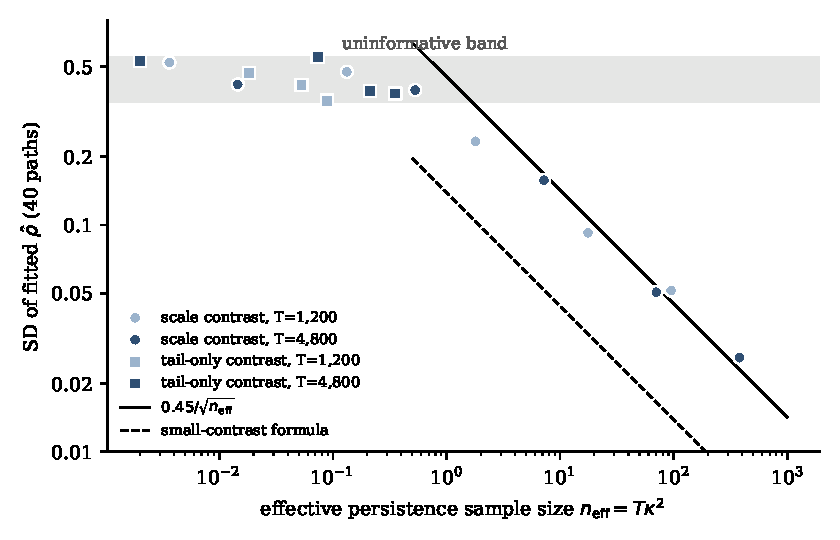
\includegraphics[width=0.72\textwidth]{collapse.pdf}
\caption{Dispersion of fitted persistence against $n_{\rm eff}=T\kappa^2$, $\rho=0.825$, 40 paths per point. Circles: volatility contrasts; squares: tail-only contrasts; light: $T=1{,}200$; dark: $T=4{,}800$. Solid: $0.45/\sqrt{n_{\rm eff}}$; dashed: Proposition~\ref{prop:small}; shaded: dispersion when persistence is not identified.}\label{fig:collapse}
\end{figure}

\subsection{Size and power of the test}\label{sec:size}
With $T=4{,}800$, $\pi_0=0.7$ and the mixture re-estimated on every path (100 paths per cell), the 5\% two-sided test rejects in 5\%, 2\% and 3\% of the paths when the regimes are independent, in two volatility designs and a tail-only design. With a volatility ratio of 2 ($\kappa=0.145$), the power is 13\%, 45\% and 93\% at $\rho=0.1$, $0.2$ and $0.4$, close to the local prediction (17\%, 52\%, 98\%). With a ratio of 1.5 ($\kappa=0.054$) it is 5\%, 7\% and 19\%. In the tail-only design ($\kappa=0.0097$) the power stays at the size level even at $\rho=0.4$. This is not a weakness of the test: as Corollary~\ref{cor:detect} shows, no test can detect persistence that the data do not contain (Supplement S3).

\paragraph{After GARCH filtering.} In a GARCH model the test is applied to standardised residuals, whose parameters are estimated. We check this with a GARCH(1,1) ($\alpha=0.07$, $\beta=0.91$) and $T=3{,}000$, re-estimating the GARCH-$t$ and the mixture on every path, and compare the $N(0,1)$ critical value with a parametric bootstrap that simulates GARCH paths with i.i.d.\ innovations from the fitted mixture. The bootstrap is evaluated with the warp-speed method of \citet{giacomini2013}, 300 paths per design. With one Student-$t$ regime the 5\% test rejects in 2.0\% of the paths with the normal critical value and 1.3\% with the bootstrap; with two independent tail regimes, in 5.0\% and 6.3\%. Filtering does not distort the test, and the normal critical value is adequate. Power is low, as the theorem predicts: 2\% with persistent tail-only regimes and 10--12\% with persistent scale regimes (ratio 1.7, $\rho=0.825$, 275 paths), because the GARCH absorbs most of the slow changes in scale. This agrees with Panel B of Table~\ref{tab:varneff}, where volatility regimes add little to a GARCH-$t$ until $T\kappa^2$ is large. The plug-in $T\hat\kappa^2$, on the contrary, is not a test: in the two null designs its 95\% quantile was 92 and 130.

\section{Empirical evidence}\label{sec:fc}

\subsection{Data and models}
We use intraday returns of WIN (B3 mini-index futures) and of a U.S.\ equity series, provisionally identified as SPY, at 1, 5, 10 and 15 minutes, and daily S\&P 500 close-to-close returns for 1990--2016 and 2000--2016 \citep{pretis2018}. Each sample is split chronologically, 80\% for estimation and 20\% for evaluation. We look at two kinds of regimes:
\begin{itemize}
\item \emph{Tail-shape regimes.} A GARCH(1,1) volatility common to both regimes, with a two-state Markov chain on the tail index of the standardised innovation (G2). We compare it with GARCH(1,1)-$t$ (G0) and with GARCH plus an i.i.d.\ two-component $t$ mixture (G1), which is G2 with $\rho=0$. On daily data G2 is also started from the fitted G1 solution, because there the original starting values ended below the G1 likelihood.
\item \emph{Volatility regimes.} An eight-parameter Student-$t$ HMM whose regimes differ in scale and tail index, with multipliers for overnight (intraday) or weekend and holiday (daily) intervals, compared with a static Student-$t$.
\end{itemize}
Details and data checks are in Supplements S4 and S5.

\subsection{Tail-shape regimes: little information, no gain}
Table~\ref{tab:dens} reports the holdout log-score differences. G2 has the highest mean log score in five of eight intraday cells and in one of the two daily samples, but none of the differences that can be tested is significant (the largest HAC statistic is 1.65). At the 90\% level, model confidence sets contain all three daily models for every score, except GARCH-$t$ at the 95\% VaR level in the 1990 sample.

\begin{table}[ht]
\centering\small
\caption{Holdout mean log-score differences of the GARCH--HMM (G2), $\times10^{-3}$ nats per return (HAC $z$ where observation-level forecasts are available)}\label{tab:dens}
\begin{tabular}{llrcc}
\toprule
Market & Frequency & Holdout $n$ & G2 $-$ G0 & G2 $-$ G1\\
\midrule
WIN & M1 & 17{,}123 & $3.42$ & $2.79$\\
U.S. & M1 & 15{,}339 & $1.10$ ($1.44$) & $0.99$ ($1.28$)\\
WIN & M5 & 3{,}412 & $0.17$ & $-0.72$\\
U.S. & M5 & 3{,}002 & $0.51$ & $0.90$\\
WIN & M10 & 1{,}694 & $-0.76$ & $-0.64$\\
U.S. & M10 & 1{,}493 & $2.25$ & $2.22$\\
WIN & M15 & 1{,}122 & $-0.05$ ($-0.02$) & $0.14$ ($0.48$)\\
U.S. & M15 & 964 & $1.35$ ($1.05$) & $0.34$ ($1.10$)\\
S\&P 500 & D1, 1990--2016 & 1{,}320 & $3.92$ ($1.65$) & $0.59$ ($0.66$)\\
S\&P 500 & D1, 2000--2016 & 814 & $2.88$ ($0.85$) & $-0.74$ ($-0.68$)\\
\bottomrule
\end{tabular}
\par\smallskip\footnotesize\emph{Notes.} G0: GARCH-$t$; G1: GARCH with i.i.d.\ $t$ mixture; G2: GARCH--HMM. Positive values favour G2. Intraday HAC: 12 lags (U.S.\ M1) or 7; daily: 20 lags.
\end{table}

The theorem explains why. On daily data, the fitted G1 mixture gives $\hat\kappa=0.066$ and $0.091$, so the estimation samples (5{,}277 and 3{,}255 returns) contain only about 23 and 27 effective observations on tail-regime persistence; with the lag-one test, only $|\rho|\gtrsim0.5$ could be detected with 80\% power. The best G2 is in fact \emph{anti}-persistent ($\hat\rho=-0.37$ and $-0.29$), with the heavy-tailed state ($\hat\nu_0\approx2.4$) almost never repeated and two parameters at their bounds. The test confirms the negative sign: the contrast autocorrelation of the standardised innovations is $-0.067$ ($Z=-4.87$) and $-0.069$ ($Z=-3.94$). Since the squared standardised innovations are also negatively autocorrelated, and the pattern remains after a GJR filter (Supplement S5), we read it as a misfit of the volatility dynamics after large shocks, not as a regime mechanism.

\subsection{Volatility regimes: enough information, better VaR}
Table~\ref{tab:var} compares the volatility-regime HMM with the static Student-$t$. At both frequencies the HMM lowers the pinball loss at all three levels, by 6 to 28\%. Here the regimes are well identified: on daily data $\hat p_{00}=0.995$, $\hat p_{11}=0.996$, the scales are 1.17 and 0.57, and $T\hat\kappa^2=139$. The daily HMM is also well calibrated (Kupiec $p=0.09$, 0.45 and 0.60), while the static model is too conservative at 99\%. Intraday, on the contrary, both models have breach rates far from nominal (Kupiec tests reject in 11 of 12 cells): a better pinball loss does not guarantee correct coverage, and calibration must always be checked separately. At both frequencies the tail index differs between regimes: the likelihood-ratio statistics for equal tails are 13.4 (WIN\$) and 64.1 (U.S.) intraday, with bootstrap $p=0.0025$, and 8.06 daily ($p=0.01$).

\begin{table}[ht]
\centering\small
\caption{Volatility-regime HMM versus static Student-$t$: holdout VaR}\label{tab:var}
\begin{tabular}{lccccc}
\toprule
 & Level & \multicolumn{2}{c}{Breaches (\%)} & Pinball gain & HAC\\
\cmidrule(lr){3-4}
Market & (\%) & Static $t$ & HMM & of HMM (\%) & $z$\\
\midrule
WIN\$ (intraday) & 95 & 7.03 & 6.00 & 9.4 & 8.82\\
WIN\$ (intraday) & 99 & 1.30 & 1.39 & 9.4 & 7.29\\
WIN\$ (intraday) & 99.5 & 0.49 & 0.70 & 7.5 & 5.43\\
U.S. (intraday) & 95 & 2.27 & 3.79 & 12.2 & 7.31\\
U.S. (intraday) & 99 & 0.25 & 0.55 & 23.1 & 11.31\\
U.S. (intraday) & 99.5 & 0.05 & 0.25 & 27.9 & 13.53\\
S\&P 500 (daily) & 95 & 4.17 & 6.06 & 5.6 & 1.61\\
S\&P 500 (daily) & 99 & 0.45 & 1.21 & 18.4 & 2.89\\
S\&P 500 (daily) & 99.5 & 0.30 & 0.61 & 27.3 & 4.39\\
\bottomrule
\end{tabular}
\par\smallskip\footnotesize\emph{Notes.} Nominal breach rates 5, 1 and 0.5\%. Pinball gain $=100(L_t-L_{\rm HMM})/L_t$; positive values favour the HMM. Intraday holdouts: 20{,}000 (WIN\$) and 15{,}444 (U.S.) returns; daily: 1{,}320 returns, 2010--2016.
\end{table}

\section{When to use regime models, limitations and future research}\label{sec:disc}

\paragraph{When can the regime model be used?} The effective sample size gives a simple rule. Fit an i.i.d.\ two-component Student-$t$ mixture to the (possibly GARCH-standardised) returns, compute $\hat\kappa$ and $n_{\rm eff}=T\hat\kappa^2$, and read it in three zones:
\begin{itemize}
\item \textbf{$T\hat\kappa^2<1$: regime information is negligible.} The sample contains less than one effective observation on persistence. The regimes may exist in the market, but this sample cannot see them: the fitted persistence is noise and the regime model will not improve the VaR. Use a static Student-$t$ or a GARCH-$t$. In our simulations this was the case for all tail-only designs, even with true persistence $\rho=0.825$.
\item \textbf{$1\le T\hat\kappa^2\lesssim50$: weak information.} Persistence starts to be estimable (the standard deviation of $\hat\rho$ is 0.23 at $T\kappa^2=2$ and 0.075 at $T\kappa^2=25$ in Table~\ref{tab:varneff}, Panel B), but the VaR gain is small: at most about 2\% over a static Student-$t$ and nothing significant over a GARCH-$t$. A GARCH-$t$ is usually enough. The daily tail-shape regimes ($T\hat\kappa^2\approx25$) fall here and gave no significant gain.
\item \textbf{$T\hat\kappa^2\gtrsim50$ and a significant test: the regime model can be used.} Persistence is well estimated and the HMM improves the VaR against both benchmarks, by an amount that grows with $T\kappa^2$: 3.3\% over the Student-$t$ and 0.6\% over the GARCH-$t$ at $T\kappa^2=60$, and 8--15\% and 1--7\% for $T\kappa^2$ between 187 and 742. The daily volatility regimes ($T\hat\kappa^2=139$) fall here and improved the VaR with correct coverage.
\end{itemize}
One caution: when there is only one regime, $\hat\kappa$ from a fitted mixture is biased upward (in simulated Student-$t$ data without regimes the median $T\hat\kappa^2$ was 11 to 57 for $T$ between 2{,}000 and 128{,}000, and after GARCH filtering its 95\% quantile was 92 to 130 at $T=3{,}000$; Section~\ref{sec:size}), so $T\hat\kappa^2<1$ is a safe conclusion, but a large $T\hat\kappa^2$ alone does not prove that regimes exist; their presence must be confirmed by the test of Section~\ref{sec:test}, which remains valid because, by Theorem~\ref{thm:persist}(iii), the persistence score is uncorrelated with the mixture scores. A bias-corrected estimator of $\kappa$ for the one-regime case, with a parametric-bootstrap reference distribution under a single Student-$t$, and a formal test of one against two regimes are being developed in ongoing work.
In every zone, fit the HMM starting also from the mixture solution, and evaluate it on a holdout with a quantile loss \emph{and} with coverage tests, because a lower loss does not guarantee correct coverage (as our intraday results show). The limits 1 and 50 are practical guides from our designs, not universal constants: the limit 1 has a direct meaning (less than one effective observation), while the limit 50 comes from Panel B of Table~\ref{tab:varneff}, where the gain over a GARCH-$t$ first becomes significant between $T\kappa^2=25$ and 60.
The code for all steps is in the online repository (\texttt{persistence\_check.py}).

\paragraph{Scope.} The exact results hold for any two-state HMM and any sample size. The simulation evidence covers twelve designs, with effective sample sizes from below 1 to 742, and the empirical evidence covers intraday and daily data from two markets. The code in the online repository runs on any return series.

\paragraph{Future research.} The regime test of this paper has a natural companion for jumps. In a second paper of the Giorno--Tsallis programme we study rare one-sided jumps that are present in the data but missing from the model. Preliminary results show three things. First, the parameters of \emph{any} fitted model move along one single direction determined by the jumps. Second, omitting 2\% downward jumps makes the 99\% VaR of GARCH, APARCH and HMM forecasts about 6--7\% too small and nearly doubles Basel yellow-zone outcomes. Third, a jump test built from the difference between downward and upward impulse scores is robust to misspecified tails (pilot size 2--3\%, power 72--77\%). Together, the two papers aim to give the risk manager two simple checks: is there a regime, and is there a jump? The test also applies after a GARCH or APARCH filter, and Theorem~\ref{thm:persist} tells us what to expect there. Because the persistence score is uncorrelated with every statistic of single returns (Theorem~\ref{thm:persist}(iii)), a static model cannot absorb omitted regime persistence: its parameters do not move. Dynamic models can, through their volatility recursion, so omitted regimes are absorbed by the dynamic parameters. Our simulations already show this for APARCH: under known regime generators, the fitted power parameter moves from about 1.0 to 1.7--1.9 with the regime design, while the asymmetry parameter stays small (Supplement S2). In the companion paper we derive a general displacement formula, $d\beta^*/d\varepsilon=H_M^{-1}\E[S_MW]$, for omitted jumps; with the persistence score in place of $W$, the same formula measures how much each APARCH parameter is distorted by omitted regimes. Other directions are the extension of Theorem~\ref{thm:persist} to more than two states, and the role of other Tsallis orders $q$ in the identification of regimes.

\section{Conclusion}
Regime models can improve Value at Risk, but only when the data contain enough information about the regimes. This paper shows that this information is measured by one simple number, $T\kappa^2$. When regimes differ in volatility, $T\kappa^2$ is large, persistence is well estimated and the VaR improves. When they differ only in tail shape, $T\kappa^2$ is small, the fitted persistence is noise and the VaR does not improve. In short: below $T\hat\kappa^2=1$ the regime information is negligible; below about 50 a GARCH-$t$ is usually enough; above about 50, and with a significant regime test, the regime model can be used for VaR. Computing $T\hat\kappa^2$ and the test of Section~\ref{sec:test} takes a few seconds, and we believe it should become a routine step before trusting a regime model for risk management.

%\section*{Funding}
%\todo{State funding, or: The author received no specific funding for this work.}

\paragraph{Data and code availability.} Code, aggregate results, the online supplement, and the 4{,}000-path manifest, seeds and per-path fits are in the repository of \citet{giorno2026code}. Market price series are not redistributed; the daily data are the \texttt{sp500data} set of the R package \texttt{gets} \citep{pretis2018}.

% References (included directly; no BibTeX needed)
\begin{thebibliography}{}

\bibitem[Alexandrovich et~al., 2016]{alexandrovich2016}
Alexandrovich, G., Holzmann, H., and Leister, A. (2016).
\newblock Nonparametric identification and maximum likelihood estimation for
  hidden {M}arkov models.
\newblock {\em Biometrika}, 103(2):423--434.

\bibitem[Bickel et~al., 1998]{bickel1998}
Bickel, P.~J., Ritov, Y., and Ryd{\'e}n, T. (1998).
\newblock Asymptotic normality of the maximum-likelihood estimator for general
  hidden {M}arkov models.
\newblock {\em Annals of Statistics}, 26(4):1614--1635.

\bibitem[Carrasco et~al., 2014]{carrasco2014}
Carrasco, M., Hu, L., and Ploberger, W. (2014).
\newblock Optimal test for {M}arkov switching parameters.
\newblock {\em Econometrica}, 82(2):765--784.

\bibitem[Cho and White, 2007]{cho2007}
Cho, J.~S. and White, H. (2007).
\newblock Testing for regime switching.
\newblock {\em Econometrica}, 75(6):1671--1720.

\bibitem[Dannemann and Holzmann, 2008]{dannemann2008}
Dannemann, J. and Holzmann, H. (2008).
\newblock Testing for two states in a hidden {M}arkov model.
\newblock {\em Canadian Journal of Statistics}, 36(4):505--520.

\bibitem[Diebold and Mariano, 1995]{diebold1995}
Diebold, F.~X. and Mariano, R.~S. (1995).
\newblock Comparing predictive accuracy.
\newblock {\em Journal of Business \& Economic Statistics}, 13(3):253--263.

\bibitem[Douc et~al., 2004]{douc2004}
Douc, R., Moulines, E., and Ryd{\'e}n, T. (2004).
\newblock Asymptotic properties of the maximum likelihood estimator in
  autoregressive models with {M}arkov regime.
\newblock {\em Annals of Statistics}, 32(5):2254--2304.

\bibitem[Giacomini et~al., 2013]{giacomini2013}
Giacomini, R., Politis, D.~N., and White, H. (2013).
\newblock A warp-speed method for conducting {M}onte {C}arlo experiments
  involving bootstrap estimators.
\newblock {\em Econometric Theory}, 29(3):567--589.

\bibitem[Giacomini and White, 2006]{giacomini2006}
Giacomini, R. and White, H. (2006).
\newblock Tests of conditional predictive ability.
\newblock {\em Econometrica}, 74(6):1545--1578.

\bibitem[Giorno, 2026]{giorno2026code}
Giorno, J. (2026).
\newblock Giorno--{T}sallis research program: replication notes and code.
\newblock \url{https://github.com/profdrgiorno/Giorno_Tsallis_paper_A}.

\bibitem[Gneiting, 2011]{gneiting2011}
Gneiting, T. (2011).
\newblock Making and evaluating point forecasts.
\newblock {\em Journal of the American Statistical Association},
  106(494):746--762.

\bibitem[Gneiting and Raftery, 2007]{gneiting2007}
Gneiting, T. and Raftery, A.~E. (2007).
\newblock Strictly proper scoring rules, prediction, and estimation.
\newblock {\em Journal of the American Statistical Association},
  102(477):359--378.

\bibitem[Gray, 1996]{gray1996}
Gray, S.~F. (1996).
\newblock Modeling the conditional distribution of interest rates as a
  regime-switching process.
\newblock {\em Journal of Financial Economics}, 42(1):27--62.

\bibitem[Haas et~al., 2004]{haas2004}
Haas, M., Mittnik, S., and Paolella, M.~S. (2004).
\newblock A new approach to {M}arkov-switching {GARCH} models.
\newblock {\em Journal of Financial Econometrics}, 2(4):493--530.

\bibitem[Hamilton, 1989]{hamilton1989}
Hamilton, J.~D. (1989).
\newblock A new approach to the economic analysis of nonstationary time series
  and the business cycle.
\newblock {\em Econometrica}, 57(2):357--384.

\bibitem[Hansen et~al., 2011]{hansen2011}
Hansen, P.~R., Lunde, A., and Nason, J.~M. (2011).
\newblock The model confidence set.
\newblock {\em Econometrica}, 79(2):453--497.

\bibitem[Kupiec, 1995]{kupiec1995}
Kupiec, P.~H. (1995).
\newblock Techniques for verifying the accuracy of risk measurement models.
\newblock {\em Journal of Derivatives}, 3(2):73--84.

\bibitem[Pretis et~al., 2018]{pretis2018}
Pretis, F., Reade, J., and Sucarrat, G. (2018).
\newblock Automated general-to-specific ({GETS}) regression modeling and
  indicator saturation for outliers and structural breaks.
\newblock {\em Journal of Statistical Software}, 86(3):1--44.

\bibitem[Qu and Zhuo, 2021]{qu2021}
Qu, Z. and Zhuo, F. (2021).
\newblock Likelihood ratio-based tests for {M}arkov regime switching.
\newblock {\em Review of Economic Studies}, 88(2):937--968.

\bibitem[R{\'e}nyi, 1959]{renyi1959}
R{\'e}nyi, A. (1959).
\newblock On measures of dependence.
\newblock {\em Acta Mathematica Academiae Scientiarum Hungaricae}, 10:441--451.

\bibitem[Ryd{\'e}n, 1994]{ryden1994}
Ryd{\'e}n, T. (1994).
\newblock Consistent and asymptotically normal parameter estimates for hidden
  {M}arkov models.
\newblock {\em Annals of Statistics}, 22(4):1884--1895.

\bibitem[Saidane and Ben~Mohamed, 2026]{saidane2026}
Saidane, M. and Ben~Mohamed, E. (2026).
\newblock Forecasting regime-dependent tail risk in digital asset portfolios
  with a mixture of hidden {M}arkov factor analyzers.
\newblock {\em Journal of Forecasting}, 45(6):2735--2759.

\bibitem[Timmermann, 2000]{timmermann2000}
Timmermann, A. (2000).
\newblock Moments of {M}arkov switching models.
\newblock {\em Journal of Econometrics}, 96(1):75--111.

\bibitem[Tsallis, 1988]{tsallis1988}
Tsallis, C. (1988).
\newblock Possible generalization of {B}oltzmann--{G}ibbs statistics.
\newblock {\em Journal of Statistical Physics}, 52:479--487.

\bibitem[Tsallis, 2009]{tsallis2009}
Tsallis, C. (2009).
\newblock {\em Introduction to Nonextensive Statistical Mechanics: Approaching
  a Complex World}.
\newblock Springer.

\bibitem[van~der Vaart, 1998]{vandervaart1998}
van~der Vaart, A.~W. (1998).
\newblock {\em Asymptotic Statistics}.
\newblock Cambridge University Press.

\end{thebibliography}

\appendix
\section{Proofs for Section~\ref{sec:persist}}\label{app:C}

\paragraph{Preliminaries.} With $c_0=\pi_1$ and $c_1=-\pi_0$ we have $\pi_0c_0+\pi_1c_1=0$ and $\bar f(1+\pi_1d)=\bar f+\pi_1(f_0-f_1)=f_0$, $\bar f(1-\pi_0d)=f_1$. Because $f_j\le\bar f/\pi_j$, $-1/\pi_1\le d\le1/\pi_0$, so $\chi<\infty$. The identity $\pi_0f_0^2+\pi_1f_1^2-\bar f^{\,2}=\pi_0\pi_1(f_0-f_1)^2$ gives $\kappa=\int(\pi_0f_0^2+\pi_1f_1^2)/\bar f-1\le\int(f_0+f_1)-1=1$, using $f_j^2/\bar f\le f_j/\pi_j$, with equality if and only if $f_0f_1=0$ almost everywhere. Since $P(K_t=0\mid Y_t=y)=\pi_0f_0(y)/\bar f(y)=\pi_0\{1+\pi_1d(y)\}$ has variance $\pi_0^2\pi_1^2\chi$, and $\mathrm{Var}\,\mathbf 1\{K_t=0\}=\pi_0\pi_1$, $\kappa$ is the squared correlation between $\mathbf 1\{K_t=0\}$ and its best predictor from $Y_t$, i.e.\ the squared maximal correlation between the binary $K_t$ and $Y_t$.

Two facts about the chain are used repeatedly. (a) $Pc=\rho c$: $(Pc)(0)=p_{00}\pi_1-(1-p_{00})\pi_0=(\pi_0+\rho\pi_1)\pi_1-(\pi_1-\rho\pi_1)\pi_0=\rho\pi_1=\rho c_0$, and similarly $(Pc)(1)=\rho c_1$. (b) $c^2=\pi_0\pi_1+(\pi_1-\pi_0)c$, as is checked at both states. Hence $V=\mathrm{span}\{1,c\}$ is invariant under $P$ and under multiplication by $c$, and $\E_\pi c=0$, $\E_\pi c^2=\pi_0\pi_1$.

\paragraph{Proof of Lemma~\ref{lem:expand}.} Conditional on the states the $Y_t$ are independent, so
\begin{align*}p(y)=\E\prod_tf_{K_t}(y_t)&=\prod_t\bar f(y_t)\,\E\prod_t\{1+c_{K_t}d(y_t)\}\\&=\prod_t\bar f(y_t)\sum_{S}m_S\prod_{t\in S}d(y_t).\end{align*}
For $S=\{t_1<\dots<t_k\}$ with gaps $h_i=t_{i+1}-t_i$, the Markov property gives \[m_S=\pi^\top MP^{h_1}M\cdots P^{h_{k-1}}M\mathbf 1,\qquad M=\mathrm{diag}(c).\] In the basis $(1,c)$ of $V$: $M1=c$, $Mc=\pi_0\pi_1\,1+(\pi_1-\pi_0)c$, $P^h1=1$, $P^hc=\rho^hc$, and $\pi^\top$ returns the coefficient of $1$. Evaluating from the right, $M\mathbf 1=c$, so the factor $P^{h_{k-1}}$ contributes $\rho^{h_{k-1}}$ to every term. On the left, $\pi^\top Mv=\pi_0\pi_1\times(\text{coefficient of }c\text{ in }v)$, so only the $c$-component after $P^{h_1}$ survives and the factor $P^{h_1}$ contributes $\rho^{h_1}$. Hence $m_\emptyset=1$, $m_{\{t\}}=\pi^\top c=0$, $m_{\{s,t\}}=\pi_0\pi_1\rho^{t-s}$, and for $k\ge3$, where $h_1$ and $h_{k-1}$ are different gaps, every monomial has degree at least $h_1+h_{k-1}\ge2$. $\square$

\paragraph{Proof of Theorem~\ref{thm:persist}.} (i)--(ii). For $g$ with finite variance, $\E[g(Y_t)\mid K_t=j]=\int g\bar f(1+c_jd)=\E_{\bar f}g+c_j\mathrm{Cov}_{\bar f}(g,d)$. The marginal law of $Y_t$ is $\bar f$, so $\mathrm{Var}\,g(Y_t)=\mathrm{Var}_{\bar f}g$. Given the states, $Y_t$ and $Y_{t+k}$ are independent, so
\begin{align*}\mathrm{Cov}\{g(Y_t),g(Y_{t+k})\}&=\mathrm{Cov}\{\E[g(Y_t)\mid K_t],\E[g(Y_{t+k})\mid K_{t+k}]\}\\&=\mathrm{Cov}_{\bar f}(g,d)^2\,\mathrm{Cov}(c_{K_t},c_{K_{t+k}})=\mathrm{Cov}_{\bar f}(g,d)^2\,\pi_0\pi_1\rho^k,\end{align*}
by (a); the same argument gives $\mathrm{Cov}\{g(Y_t),h(Y_{t+k})\}=\pi_0\pi_1\rho^k\mathrm{Cov}_{\bar f}(g,d)\mathrm{Cov}_{\bar f}(h,d)$. The Cauchy--Schwarz inequalities $\mathrm{Cov}_{\bar f}(g,d)^2\le\mathrm{Var}_{\bar f}(g)\chi$ and $\mathrm{Cov}_{\bar f}(h,d)^2\le\mathrm{Var}_{\bar f}(h)\chi$, each with equality if and only if the function is affine in $d$, give (ii); when $\rho\neq0$ equality in (ii) also requires both covariances to be nonzero, i.e.\ nonzero slopes, and when $\rho=0$ both sides vanish. For $g=d$, $\E_{\bar f}d=\int(f_0-f_1)=0$ and $\mathrm{Cov}_{\bar f}(d,d)=\chi$, so the correlation is $\pi_0\pi_1\chi\rho^k=\kappa\rho^k$.

(iii). By the lemma, $p/\prod\bar f$ is a polynomial in $\rho$ that equals 1 at $\rho=0$, because every $m_S$ with $|S|\ge2$ has positive degree; the HMM with $\rho=0$ is the independent mixture for every $(\pi_0,f_0,f_1)$. The derivative at $\rho=0$ retains only monomials of degree one, which occur only for $S=\{t,t+1\}$, giving \eqref{eq:pscore}. Under $\rho=0$ the $Y_t$ are i.i.d.\ with density $\bar f$, $\E d=0$ and $\E d^2=\chi$. Two products $d(Y_t)d(Y_{t+1})$ and $d(Y_s)d(Y_{s+1})$ with $s\neq t$ share at most one index, so their covariance contains an isolated mean-zero factor and vanishes; hence $\mathrm{Var}\,S_{\rho,T}=(\pi_0\pi_1)^2(T-1)\chi^2=(T-1)\kappa^2$. For any $g$ with $\E_{\bar f}g^2<\infty$ and any $u$, $\E[d(Y_t)d(Y_{t+1})g(Y_u)]=0$, since at least one of $t,t+1$ differs from $u$ and that factor is independent of the others with mean zero. The scores of the independent-mixture parameters $\theta$ are sums $\sum_u\partial_\theta\log\bar f_\theta(Y_u)$, so the cross-information $I_{\rho\theta}$ is zero and the efficient information equals $I_{\rho\rho}=(T-1)\kappa^2$. $\square$

\paragraph{Proof of Corollary~\ref{cor:detect}.} Under local asymptotic normality with information $\kappa^2$ per observation (part~(iii)), the experiments $\{P_{h/\sqrt T}\}$ converge to the Gaussian shift experiment with mean $h\kappa^2$ and variance $\kappa^2$, and the asymptotic power envelope for one-sided tests at level $\alpha$ is $1-\Phi(z_{1-\alpha}-h\kappa)$ \citep[Ch.~15]{vandervaart1998}. When the mixture family is identifiable, the nuisance parameters are $\sqrt T$-consistently estimable under the null, and because their scores are orthogonal to \eqref{eq:pscore}, plug-in estimation does not change the score test's limit; it therefore attains the envelope. For a fixed $\rho$, $\E\{d(Y_t)d(Y_{t+1})\}=\pi_0\pi_1\rho\chi^2$ by part~(i), so the standardised lag-one statistic has mean $\sqrt{T-1}\,\kappa\rho$; setting this equal to $z_{1-\alpha}+z_{1-\beta}$ gives the first threshold. In the small-contrast regime the Kullback--Leibler rate between the HMM and the independent mixture is $G$ of Proposition~\ref{prop:small}, so the log-likelihood-ratio test has noncentrality $(2TG)^{1/2}=\{T\kappa^2\rho^2/(1-\rho^2)\}^{1/2}$, which gives the second. $\square$

\paragraph{Sketch of proof of Proposition~\ref{prop:small}.} Write the likelihood through its predictive decomposition, $p(y_{1:T})=\prod_t\bar f(y_t)\{1+m_td(y_t)\}$ with $m_t=\E[c_{K_t}\mid Y_{1:t-1}]$, so that the score is the martingale sum $\partial_\rho\log p=\sum_t\partial_\rho m_t\,d(Y_t)/\{1+m_td(Y_t)\}$. With $d=\delta a$ and $\delta\to0$, the filter is linear to leading order: $\E[d(Y_s)\mid K_s]=c_{K_s}\chi$, $\mathrm{Cov}(c_{K_t},d(Y_s))=\pi_0\pi_1\rho^{t-s}\chi$ and $\mathrm{Cov}(d(Y_s),d(Y_u))=\chi\mathbf 1\{s=u\}+O(\delta^4)$, so $m_t=\pi_0\pi_1\sum_{s<t}\rho^{t-s}d(Y_s)+O_p(\delta^2)$. The $O_p(\delta^2)$ remainder comes from the Bayes update, a term proportional to $(\pi_1-\pi_0)\rho\,m_{t-1}d(Y_{t-1})$, and vanishes when $\pi_0=\pi_1$; it changes the results below only at order $\delta^5$. Hence $\partial_\rho m_t=\pi_0\pi_1\sum_{s<t}(t-s)\rho^{t-s-1}d(Y_s)+O_p(\delta^2)$, and the per-step conditional variance of the score increment is $\chi\,\E(\partial_\rho m_t)^2\to\kappa^2\sum_{h\ge1}h^2\rho^{2(h-1)}=\kappa^2(1+\rho^2)/(1-\rho^2)^3$ at order $\delta^4$, using $\sum_{h\ge1}h^2x^{h-1}=(1+x)/(1-x)^3$. For the forecast gain, the expected one-step gain over $\bar f$ is the Kullback--Leibler divergence $\int\bar f(1+m_td)\log(1+m_td)=\tfrac12m_t^2\chi+O(|m_t|^3\delta^3)$, and $\E m_t^2\to(\pi_0\pi_1)^2\chi\rho^2/(1-\rho^2)$ at order $\delta^2$, so $G=\tfrac12\kappa^2\rho^2/(1-\rho^2)+o(\delta^4)$. A complete proof requires bounds on the remainders that are uniform in $t$; we do not provide them. Monte Carlo checks with an exact forward filter (a three-point base density, $\pi_0=0.3$, $\rho=0.7$, $T=2{,}000$, 4{,}000 paths; script \texttt{small\_contrast\_check.py}) give simulated-to-predicted ratios of 0.87, 0.96 and 0.996 for the information and 0.97, 0.99 and 0.997 for the gain at $\delta=0.4$, $0.2$ and $0.1$, consistent with the leading terms and with slow convergence at large $\rho$.
\end{document}
